\documentclass{beamer}

\usepackage[utf8]{inputenc}
\usecolortheme{beaver}
\usepackage{caption}
\usepackage{subcaption}
\usepackage{mathtools}
\usepackage{todonotes}
\usepackage{amsmath}
\usepackage{bm}
\usepackage{listings}
\usepackage{ragged2e}
\usepackage{fancyvrb}

\def\ci{\perp\!\!\!\!\!\perp}

\tikzstyle{latent} = [ draw, circle, inner sep = 2pt, minimum size = 0.65cm ]
\tikzstyle{observed} = [ draw, rectangle, inner sep = 2pt, minimum size = 0.65cm ]
\tikzstyle{tikztext} = [ draw, inner sep = 2pt, minimum size = 0.65cm, rounded corners=0.1cm ]

\newtheorem{proposition}{Proposition}

\setbeamertemplate{section in toc}{\inserttocsectionnumber.~\inserttocsection}
\usetheme{Boadilla}
\makeatletter
\setbeamertemplate{footline}{%
    \leavevmode%
    \hbox{%
        \begin{beamercolorbox}[wd=.3\paperwidth,ht=2.25ex,dp=1ex,center]{author in head/foot}%
            \usebeamerfont{author in head/foot}\insertshortauthor\expandafter\beamer@ifempty\expandafter{\beamer@shortinstitute}{}{~~(\insertshortinstitute)}
        \end{beamercolorbox}%
        \begin{beamercolorbox}[wd=.55\paperwidth,ht=2.25ex,dp=1ex,center]{title in head/foot}%
            \usebeamerfont{title in head/foot}\insertshorttitle
        \end{beamercolorbox}%
        \begin{beamercolorbox}[wd=.15\paperwidth,ht=2.25ex,dp=1ex,right]{date in head/foot}%
            \usebeamerfont{date in head/foot}\insertshortdate{}\hspace*{2em}
            \insertframenumber{} / \inserttotalframenumber\hspace*{2ex} 
        \end{beamercolorbox}}%
        \vskip0pt%
    }
\makeatother

\begin{document}

\title[Combining Graphical and Algebraic Approaches for Parameter Identification in Latent Variable SEM]{Combining Graphical and Algebraic Approaches for Parameter Identification in Latent Variable Structural Equation Models}
\author {Ankur Ankan \and Inge Wortel \and Kenneth A. Bollen \and Johannes Textor}
\institute[]{Radboud University, Netherlands}
\date{}
\maketitle

\section{Overview}
\begin{frame}
	\frametitle{Parameter Identification}
	\todo[inline]{Add Bollen's institute}
	\begin{block}{Problem Statement}
		Given a DAG $ G = (V, E) $ and an observational dataset on $ V $, is the causal effect
		of $ \bm{X} \in V $ on $ \bm{Y} \in V $ estimable?
	\end{block}
	\begin{figure}
		\centering
		\begin{subfigure}{0.5 \textwidth}
			\centering
			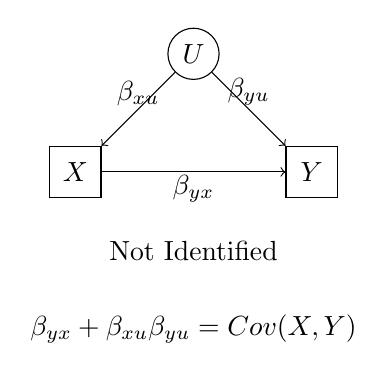
\begin{tikzpicture}
				\tikzstyle{every node}=[align=center, inner sep=1pt]
				\node[latent] (u) at (1.5, 1.5) {$ U $};
				\node[observed] (x) at (0, 0) {$ X $};
				\node[observed] (y) at (3, 0) {$ Y $};
				\draw[->] (u) -- (x) node[midway, above]{$ \beta_{xu} $};
				\draw[->] (u) -- (y) node[midway, above]{$ \beta_{yu} $};
				\draw[->] (x) -- (y) node[midway, below]{$ \beta_{yx} $};
				\node at (1.5, -1) {Not Identified};
				\node at (1.5, -2) {$\beta_{yx} + \beta_{xu} \beta_{yu} = Cov(X, Y) $};
			\end{tikzpicture}
		\end{subfigure}%
		\begin{subfigure}{0.5 \textwidth}
			\centering
			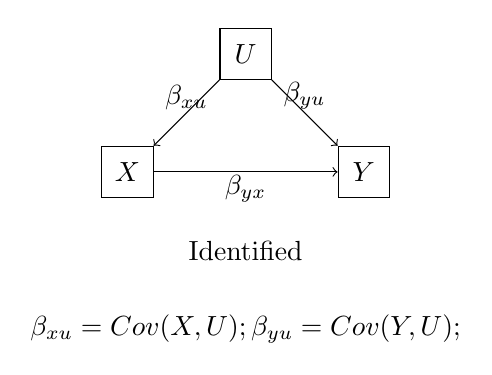
\begin{tikzpicture}
				\tikzstyle{every node}=[align=center, inner sep=1pt]
				\node[observed] (u) at (1.5, 1.5) {$ U $};
				\node[observed] (x) at (0, 0) {$ X $};
				\node[observed] (y) at (3, 0) {$ Y $};
				\draw[->] (u) -- (x) node[midway, above]{$ \beta_{xu} $};
				\draw[->] (u) -- (y) node[midway, above]{$ \beta_{yu} $};
				\draw[->] (x) -- (y) node[midway, below]{$ \beta_{yx} $};
				\node at (1.5, -1) {Identified};
				\node at (1.5, -2) {$ \beta_{xu} = Cov(X, U); \beta_{yu} = Cov(Y, U); $};
			\end{tikzpicture}
		\end{subfigure}
	\end{figure}
\end{frame}

% \begin{frame}
% 	\frametitle{Identification}
% 	\begin{block}{Pearl's do-calculus}
% 		do-calculus can give formulas on observed distribution for 
% 		every possible identifiable parameter.
% 	\end{block}
% 	\begin{itemize}
% 		\item But no efficient algorithm for checking identifablity using
% 			do-calculus.
% 		\item Different criteria have been proposed which can identify 
% 			parameters in special cases.
% 		\item For example Back-door criterion, front-door criterion etc.
% 		\item Another method for identification is the IV based estimation 
% 			method
% 	\end{itemize}
% \end{frame}

\begin{frame}
	\frametitle{Identifiability using Instrumental Variables(IV)}
	\begin{block}{Instrumental Variable}
		A variable $ Z $ is an IV for estimating the effect $ X \rightarrow Y $
		if $ Z $ is d-connected to $ X $ and all open paths to $ Y $ go through
		$ X $.
	\end{block}
	\todo[inline]{Replace this with a better definition.}
	\begin{figure}
		\centering
		\begin{subfigure}{0.5\linewidth}
			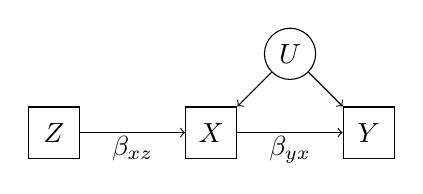
\begin{tikzpicture}
				\tikzstyle{every node}=[align=center, inner sep=1pt]
				\node[observed] (z) at (0, 0) {$ Z $};
				\node[observed] (x) at (2, 0) {$ X $};
				\node[observed] (y) at (4, 0) {$ Y $};
				\node[latent] (u) at (3, 1) {$ U $};
				\draw[->] (z) -- (x) node[midway, below] {$ \beta_{xz} $};
				\draw[->] (x) -- (y) node[midway, below] {$ \beta_{yx} $};
				\draw[->] (u) -- (x);
				\draw[->] (u) -- (y);
			\end{tikzpicture}
		\end{subfigure}%
		\begin{subfigure}{0.5\linewidth}
			$$ \beta_{yx} = \frac{Cov(Y, Z)}{Cov(Z, X)} = \frac{\beta_{yx} \beta_{xz}}{\beta_{xz}}$$
		\end{subfigure}
	\end{figure}
	\begin{block}{Instrumental Set Criterion}
	\end{block}
\end{frame}

\begin{frame}
	\frametitle{Structural Equation Models}
	\begin{itemize}
		\item In DAG literature, the effect being estimated is between two
			observed variables.
		\item This is rarely the case in Latent Variable SEMs where we usually
			assume a latent underlying structure and observed variables
			act as measurements for the latents.
		\item Similar to the DAG literature, SEMs literature has a IV 
			identification criterion called Model Implied Instrumental 
			Variables (MIIV).
		\item The main ideas behind MIIV approach is scale setting and Latent-
			to-observed transformation.
	\end{itemize}
\end{frame}

\begin{frame}
	\frametitle{Overview}
	\begin{figure}
		\centering
		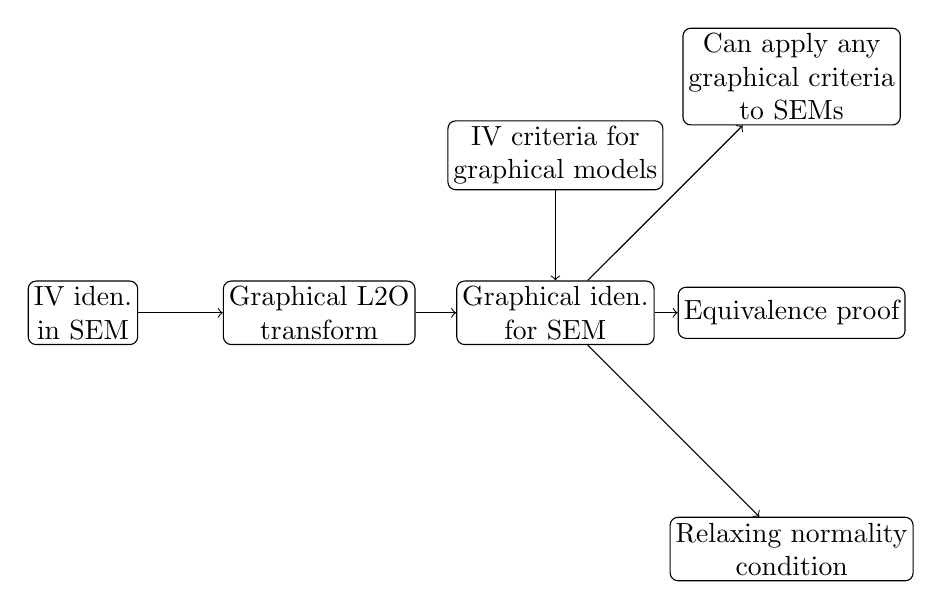
\begin{tikzpicture}
			\tikzstyle{every node}=[align=center, inner sep=1pt]
			\node[tikztext] (ivdag) at (6, 2) {IV criteria for \\ graphical models};
			\node[tikztext] (ivsem) at (0, 0) {IV iden. \\ in SEM};
			\node[tikztext] (graphl2o) at (3, 0) {Graphical L2O \\ transform};
			\node[tikztext] (graphidden) at (6, 0) {Graphical iden. \\ for SEM};
			\node[tikztext] (graphcri) at (9, 3) {Can apply any \\ graphical criteria \\ to SEMs};
			\node[tikztext] (equival) at (9, 0) {Equivalence proof};
			\node[tikztext] (normal) at (9, -3) {Relaxing normality \\ condition}; 
			\draw[->] (ivsem) -- (graphl2o);
			\draw[->] (ivdag) -- (graphidden);
			\draw[->] (graphl2o) -- (graphidden);
			\draw[->] (graphidden) -- (graphcri);
			\draw[->] (graphidden) -- (equival);
			\draw[->] (graphidden) -- (normal);
		\end{tikzpicture}
	\end{figure}
\end{frame}

\begin{frame}
	\frametitle{Graphical Approach}
	\begin{block}{Instrumental Set Criterion (Brito and Pearl 2002)}
Given an ADMG $\cal
	G$, a variable $y$, and a subset $X$ of the parents of $y$, 
	a set of variables
	$I$ fulfills the 
	\emph{instrumental set condition}
	if for {some} permutation $ i_1 \ldots i_k $ of
	$ I $ and {some} permutation
	$ x_1 \ldots x_k $ of $ X $ we have: 
	\begin{enumerate}
		\item There are no treks from $I$ to $y$ in the graph ${\cal
			G}_{\overline{X}}$ obtained by removing all arrows 
			between $X$ and $y$. 
		\item For each $j$, $1 \leq j \leq k$, there is a trek $\pi_j$ from
			$I_j$ to $X_j$ such that for all $i < j$: (1) $I_i$ does not
			occur on any trek $\pi_j$; and (2) all intersections between
			$\pi_i$ and $\pi_j$ are on the left side of $\pi_i$ and the
			right side of $\pi_j$.
	\end{enumerate}
	\end{block}
\end{frame}

\begin{frame}
	\frametitle{Why can't we directly apply graphical criteria to SEMs}
	\begin{itemize}
		\item Criterion have been developed assuming that the parameters 
			begin identified are between observed variables.
		\item Show an example of a SEM where we are looking to identify 
			the parameter on latent variables.
	\end{itemize}
\end{frame}

\begin{frame}
	\frametitle{MIIV Approach}
	\begin{itemize}
		\item The MIIV approach deals with these cases by doing a
			Latent-to-Observed (L2O) transformation.
	\end{itemize}
\end{frame}

\begin{frame}
	\frametitle{The proposed graphical transformation}
	The proposed graphical transformation is analogous to the algebraic 
	transformation such that it makes edges between observed variables
	with the path coefficient we want to estimate.
\end{frame}

\begin{frame}
	\frametitle{Examples}
		\begin{figure}[t]
		    \centering
		    \begin{subfigure}[b]{.33\linewidth}
		    	\centering
			\includegraphics[scale=0.6, page=4]{figures-inge.pdf}
		        \caption{}
			\label{fig:l2o_parent}
		    \end{subfigure}%
		    \begin{subfigure}[b]{.33\linewidth}
		    	\centering
			\includegraphics[scale=0.6, page=5]{figures-inge.pdf}
		        \caption{}
			\label{fig:l2o_child}
		    \end{subfigure}%
		    \begin{subfigure}[b]{.33\linewidth}
		    	\centering
			\includegraphics[scale=0.6, page=6]{figures-inge.pdf}
		        \caption{}
			\label{fig:l2o_both}
		    \end{subfigure}
			\caption{Example L2O transformations for path
			coefficients (a) from a latent to an observed variable;
			(b) from an observed to a latent variable; (c) between
			two latent variables.}
		\end{figure}
\end{frame}

\end{document}
